% \section{Désassemblage}
Le désassemblage est l'opération inverse de l'assemblage : il consiste à récupérer le code assembleur source du binaire.
Cette tâche semble particulièrement simple puisque l'assemblage consiste simplement à trouver les octets correspondants à chaque instruction à l'aide de la documentation officielle du processeur puis à mettre en forme le fichier binaire en remplissant correctement ses entêtes et ses sections.
Pourtant on a vu que, dans le modèle de Harvard modifié, les données et le code peuvent être mêlés. 
En particulier les parties de données (comme la section \pdata) peuvent être exécutées. 
De même les sections de code peuvent contenir des informations destinées à être simplement lues ou modifiées mais jamais exécutées.
La difficulté du désassemblage consiste donc à séparer les parties potentiellement exécutables des données.

Ainsi un désassemblage à priori cohérent de \helloworld\ consisterait à considérer les deux sections comme contenant du code potentiellement exécutable. Ce désassemblage sera composé de la section \ptext\ déjà désassemblé Figure \ref{fig:text_helloworld} et la section \pdata\ donnée Figure \ref{fig:data_exec_helloworld}.
Ce désassemblage n'est pas correct et on peut le prédire. 
On connaît le point d'entrée du binaire, qui est l'adresse \texttt{8048080} dans la section \ptext.
Les instructions exécutées dans la section \ptext\ à la suite du point d'entrée sont séquentielles et ne peuvent détourner l'exécution vers la section \pdata. 
Le code désassemblé dans cette section n'est donc pas atteignable. Dans ce cas on sait alors que la section \pdata\ ne contient pas de code et ne doit pas être désassemblée.

\begin{figure}
\begin{center}
\begin{tabular}{|c|c|l|l|}
\hline
Emplacement & Adresses de chargement & Octets & Instruction\\ 
dans le fichier & &  & \\ 
\hline
94 & 80490a4 & 48    & dec    eax			\\
95 & 80490a5 & 65    & gs				\\
96 & 80490a6 & 6c    & ins    BYTE PTR es:[edi],dx	\\
97 & 80490a7 & 6c    & ins    BYTE PTR es:[edi],dx	\\
98 & 80490a8 & 6f    & outs   dx,DWORD PTR ds:[esi]	\\
99 & 80490a9 & 2c 20 & sub    al,0x20			\\
9b & 80490ab & 77 6f & ja     0x804911c			\\
9d & 80490ad & 72 6c & jb     0x804911b			\\
9f & 80490af & 64    & fs				\\
a0 & 80490b0 & 0a    & .byte 0xa			\\
\hline
\end{tabular}
\end{center}
\caption{Section \pdata\ de \helloworld\ désassemblée comme du code}
\label{fig:data_exec_helloworld}
\end{figure}

% \paragraph{Utilisation de sauts dynamiques.}
En pratique un programme est constitué d'un grand nombre d'instructions de saut et notamment de sauts dynamiques de type \texttt{jmp eax}.
Ce type d'instructions posent un souci lors de l'analyse : sans connaître précisément la ou les valeurs potentielles d'\eax, impossible de prédire la cible du saut et donc de savoir le code potentiellement exécuté à la suite de cette instruction.
Dans l'exemple du \helloworld, si une telle instruction est présente dans la section \ptext, il devient difficile d'exclure l'exécution possible de code dans la section \pdata.

\section{Difficulté théorique du désassemblage.}
~\\\ijym{reprendre la preuve}
\itodo{Pb de l'arrêt: il existe HALT / HALT(P) = 1 ssi quelle que soit l'entrée I, P(I) termine ?}
\itodo{Pb du désassemblage : borne min : intersection de CODE(P,I), borne max : union}
\itodo{borne min ~ arrêt ?}
On a vu que le problème du désassemblage tient dans la difficulté de séparer les parties de code potentiel des parties de données.
Plus précisément le but du désassemblage d'un programme P est alors de déterminer l'ensemble des adresses $a$ du programme pour lesquelles il existe une entrée I telle que l'exécution de P(I) atteint $a$.
Nous citons ici un argument tiré de la thèse de Joan Calvet \cite{Calvet2013} montrant le caractère indécidable de ce problème en réduisant le problème de l'arrêt à celui-ci.

Supposons que le problème soit décidable et notons $CODE$ le programme tel que, pour tout programme P, $CODE(P)$ est l'ensemble des adresses des instructions de P atteignables lors de l'exécution de P. Pour tout programme P et toute entrée I à P, on peut définir le programme P' suivant qui ne prend pas d'entrée :

\begin{center}
\begin{tabular}{|l|l|}
\hline
Adresse & Commande \\
\hline
0 & P(I)\\
% $\alpha$ & halt \\
\hline
\end{tabular}
\end{center}

On remarque que $CODE(P')$ contient exactement les adresses des instructions de P 
Deux cas sont alors possibles.
\begin{itemize}
 \item Soit il existe $\alpha\in CODE(P')$ tel que l'instruction à l'adresse $\alpha$ est l'instruction d'arrêt \texttt{halt} et dans ce cas l'exécution atteint l'adresse $\alpha$ donc le programme P termine sur l'entrée I.
 \item Dans le cas contraire aucune instruction d'arrêt n'est atteignable et donc le programme P ne termine pas sur l'entrée I.
\end{itemize}
\begin{itemize}
 \item Soit $\alpha\in\ CODE(P')$ et dans ce cas l'exécution atteint l'adresse $\alpha$ donc le programme P termine sur l'entrée I.
 \item Soit $\alpha\notin\ CODE(P')$ donc le programme P ne termine pas sur l'entrée I.
\end{itemize}
~\\
On en déduit donc que le désassemblage permet de résoudre le problème de l'arrêt qui est pourtant connu pour être indécidable ; c'est absurde.
Ainsi le problème du désassemblage est indécidable.


\section{Reconstruction du graphe de flot de contrôle (GFC).}
Nous avons vu jusqu'ici une réprésentation des programmes assembleur et binaires sous forme de code linéaire mais il est plus aisé de visualiser les programmes à l'aide d'un graphe de flot de contrôle (GFC).
Ce graphe représente les instructions sous forme de sommets et les sauts du flot de contrôle d'une instruction à une autre sous forme d'arcs.
Prenons le programme assembleur donné en figure \ref{fig:asm_eax_code}. Il ne fait que modifier le registre \eax, effectue des sauts selon la valeur d'\eax\ et se termine avec une valeur pour \eax\ à 1 ou 2. L'instruction \texttt{mov eax, 3} n'est pas atteignable puisqu'elle suit un saut inconditionnel et qu'aucune autre instruction ne provoque un saut vers elle.
Ainsi le graphe de flot de contrôle de ce programme est celui donné en figure \ref{fig:asm_eax_cfg}.

Le sommet coloré en orange est le point d'entrée du programme. Dans le cas où le flot de contrôle peut passer de l'instruction $a$ à l'instruction $b$, l'arc entre $a$ et $b$ est en noir si $b$ suit $a$ en mémoire et en rouge sinon, c'est à dire dans le cas où il s'agit d'un saut.

Un graphe de flot idéal inclut exactement l'ensemble des instructions atteignables dans le programme et un arc ne relie deux instructions que s'il existe au moins une exécution du programme dans laquelle les deux instructions sont exécutées consécutivement.
\\

\begin{figure}
\begin{center}
\subfigure[Code assembleur]{
\begin{tabular}[b]{|l|l|l|}
\hline
Adresse & Octets & Instruction\\ 
\hline
 8048067  &  b8 00 00 00 00         &  mov    eax,0x0 \\
 804806c  &  eb 05                  &  jmp    0x8048073 \\
 804806e  &  b8 03 00 00 00         &  mov    eax,0x3 \\
 8048073  &  83 f8 00               &  cmp    eax,0x0 \\
 8048076  &  74 06                  &  je     0x804807e \\
 8048078  &  b8 01 00 00 00         &  mov    eax,0x1 \\
 804807d  &  c3                     &  ret     \\
 804807e  &  b8 02 00 00 00         &  mov    eax,0x2 \\
 8048083  &  c3                     &  ret     \\
\hline
\end{tabular}
\label{fig:asm_eax_code}
}
\subfigure[Graphe de flot de contrôle]{
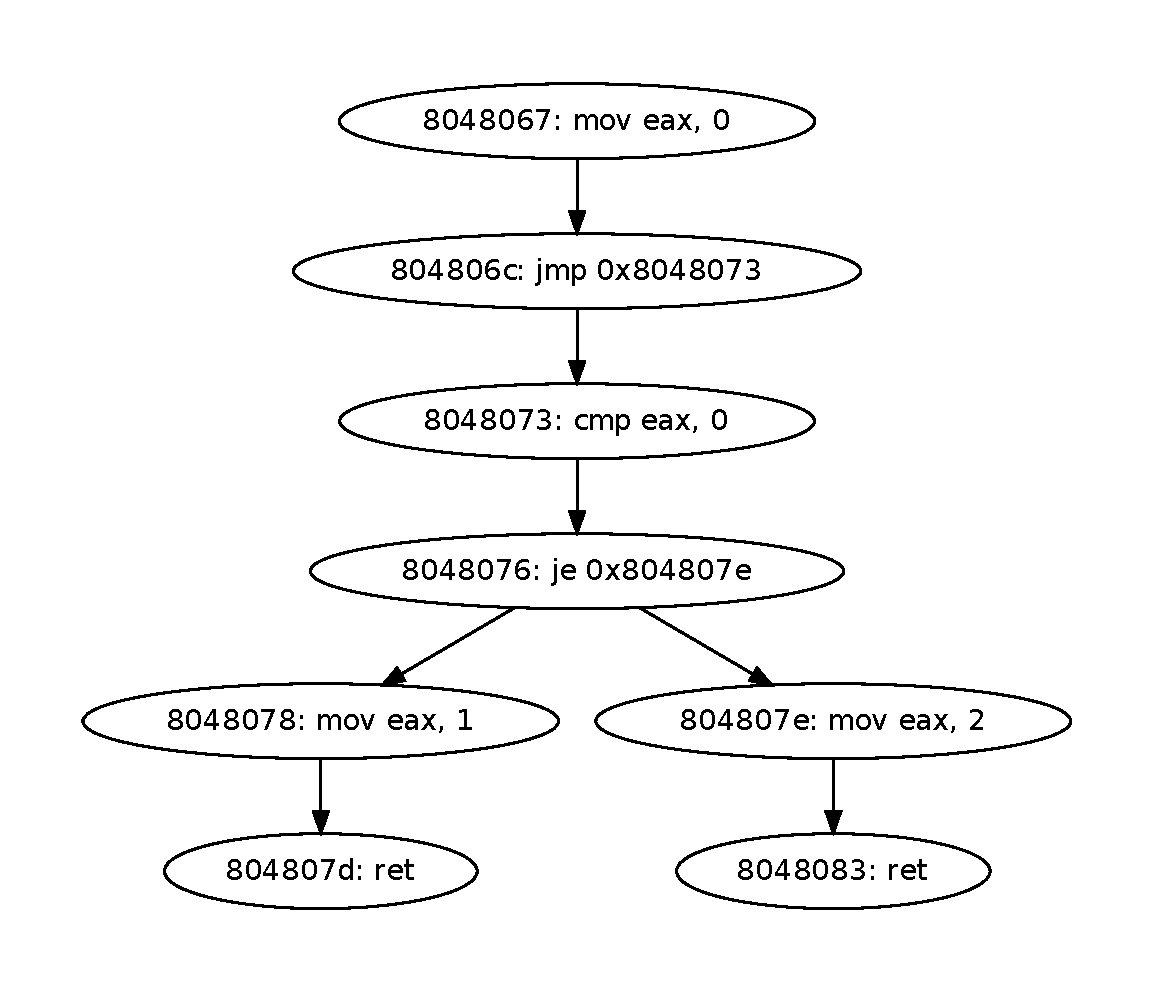
\includegraphics[width=0.6\textwidth]{supports/eax-cfg/eax.pdf}
\label{fig:asm_eax_cfg}
}
\end{center}
\caption{Représentation d'une fonction assembleur modifiant \eax}
\label{fig:asm_eax}
\end{figure}

% \subsection{Approche statique}
% \todo[inline]{Avantages et inconvénients des deux (couverture, précision, complétude)\\
% Exemple sur les programmes donnés}
\section{Revue de littérature}
\subsection{Parcours linéaire}
Un désassemblage suivant un parcours linéaire désassemble, pour chaque section, la première instruction à l'adresse $a$ puis l'instruction à l'adresse $a+k$ où $k$ est le nombre d'octets sur lesquels l'instruction est codée.
Ainsi pour une suite d'instructions séquentielles cette méthode suit le flot de contrôle mais si une instruction de type \jmp\ est rencontrée, le désassemblage s'intéressera à l'instruction qui suit en mémoire et non celle qui sera logiquement exécutée ensuite.
La figure \ref{fig:asm_eax_code} donne un exemple de désassemblage linéaire d'une fonction assembleur.
L'avantage de cette technique réside dans sa simplicité et le fait qu'elle couvre l'ensemble de la mémoire.
Pourtant, ne cherchant pas à suivre le flot de contrôle, elle ne permet pas de séparer le code exécutable des données et désassemble des instructions qui ne sont pas atteignables comme l'instruction \mov\ à l'adresse $804806e$ de la figure \ref{fig:asm_eax}.
C'est l'approche utilisée par le désassembleur standard du projet GNU, objdump \cite{objdump}.
\todo[inline]{radare?}

\subsection{Parcours récursif}
À l'inverse du parcours linéaire, le parcours récursif suit le flot de contrôle et désassemble les instructions qui se suivent logiquement en partant du point d'entrée du programme. Le graphe de flot de contrôle peut être déduit du parcours récursif : la figure \ref{fig:asm_eax_cfg} donne celui de l'exemple précédent.
Une telle approche est utilisée par le désassembleur commercial IDA \cite{IDA}.
L'avantage de cette technique est qu'elle ne désassemble que des instructions dont on peut raisonnablement penser qu'elles sont atteignables.

Cependant certains chemins ne sont pas atteignables en raison de variables définies. 
L'instruction à l'adresse \texttt{8048076} provoque un saut vers l'adresse \texttt{804807e} si la comparaison effectuée à l'instruction précédente est vraie, c'est à dire si $\eax=0$, et saute vers l'adresse \texttt{8048078} dans le cas contraire.
Or la première instruction de la fonction donne à \eax\ la valeur 0. Dans tous les cas le saut se produira donc vers l'adresse \texttt{804807e} et l'autre branche n'est pas atteignable.

D'autre part si des sauts dynamiques sont utilisés comme avec l'instruction \texttt{jmp eax}, le parcours récursif s'arrête alors qu'il est clair que d'autres instructions seront exécutées.
\jym{déterminer eax peut être indécidable // le pb vient des embranchements et des prédicats opaques ?}


\subsection{Parcours spéculatif}
Pour pallier à l'incomplétude d'un parcours récursif, un parcours spéculatif a été proposé pour les parties de mémoire non désassemblées par l'approche récursive. 
Il s'agit d'effectuer un parcours linéaire sur ces zones mémoires et d'utiliser des heuristiques pour déterminer s'il s'agit de code ou de données.
Les heuristiques proposées portent par exemple sur la détection de fonctions assembleur \cite{KruegelRVV04}, repérables grâce à une suite d'instructions caractéristiques. Une autre approche évalue la probabilité qu'une suite d'instructions soit effectivement du code en apprenant au préalable des suites d'instructions réelles lancées lors de l'exécution de programmes \cite{KDF09}.
\ijym{+ de biblio}

% \subsection{Approche dynamique}

% \paragraph{Décompilation.}

\section{Analyse statique et dynamique}
Dans le domaine de l'analyse de code, on parle d'analyse dynamique lorsque le fichier binaire à analyser est exécuté au moins partiellement et que l'analyse consiste à observer une ou des exécutions du programme. Au contraire lors d'une analyse statique on cherche à inférer des propriétés sur le programme sans l'exécuter.

Les deux techniques permettent de récupérer du code assembleur à partir du programme et donc de réaliser un désassemblage et de reconstruire un graphe de flot de contrôle.
L'avantage de l'analyseur dynamique est que, puisqu'il travaille sur une exécution spécifique du programme, il est précis : les instructions qui sont exécutées doivent être inclues dans le désassemblage.
Par contre il n'est pas complet vu qu'il ne suivra pas des branches du programme qui pourraient être utilisées si leurs conditions étaient vérifiées. À l'inverse un analyseur statique n'est pas précis et ne peut en général pas être complet à cause de l'impossibilité de prédire certaines cibles de sauts dynamiques.